\documentclass[fleqn,10pt]{wlscirep}
\usepackage[utf8]{inputenc}
\usepackage[T1]{fontenc}
\usepackage{listings}
\usepackage{xcolor}
\usepackage{booktabs}
\usepackage{float}
\usepackage{fancyhdr}
\usepackage{caption}
\usepackage{graphicx}

\graphicspath{ {./} }

\pagestyle{fancy}
\fancyhf{}
\fancyhead[LE,RO]{Dharak Vasavda}
\fancyhead[RE,LO]{Parallel Binary Search with OpenMP}
\fancyfoot[LE,RO]{\thepage}

\renewcommand{\headrulewidth}{2pt}
\renewcommand{\footrulewidth}{1pt}

\DeclareCaptionFont{white}{\color{white}}
\DeclareCaptionFormat{listing}{\colorbox{gray}{\parbox{\textwidth}{#1#2#3}}}
\captionsetup[lstlisting]{format=listing,labelfont=white,textfont=white}
\captionsetup{justification=raggedright,singlelinecheck=false}

% This concludes the preamble

\title{Parallel Binary Search Using OpenMP}

\author{Dharak Vasavda}
\affil{$d\_vasavda@u.pacific.edu$}


%\keywords{Keyword1, Keyword2, Keyword3}



\begin{document}


\maketitle
\flushbottom
\pagebreak
\raggedbottom


\section{Problem}
Binary Search is a divide-and-conquer searching algorithm which searches for an input value in a sorted array. The average-case time complexity for Binary Search is $\mathcal{O}(log{}n)$. Considering that it is a divide-and-conquer search where the input array is repeatedly divided into equal halves, can the search operation be made even faster using OpenMP parallelization?

\subsection*{Prior Solutions}
Parallel Binary Search implementations with OpenMP do exist, however; rarely is there any specifically real-world timing data comparison between a serial and parallel implementation. Due to such circumstance, this scientific paper aims to compare the real-world performance between a parallel and serial implementation. It also aims to investigate any real-world performance differences between a serial and parallel approach to Binary Search.

\section{Design}
\subsection*{Typical Serial Binary Search}
Typically, a serial approach to non-recursive Binary Search algorithm goes as follows:

\begin{lstlisting}[language=C, caption=Serial Binary Search]
    while (first <= last) {
        int middle = first + (last - first) / 2;

        // Check if search value is present at middle
        if (randomNums[middle] == searchVal)
            return middle;

        // If search value greater, ignore left half
        if (randomNums[middle] < searchVal) {
            first = middle + 1;
        }

        // If search value is smaller, ignore right half
        else
            last = middle - 1;
    }
\end{lstlisting}

\pagebreak


\subsection*{Parallel Binary Search Design}
The sample code block below may assist with understanding the parallel solution.

\begin{lstlisting}[language=C, caption=OpenMP Binary Search]
#pragma omp parallel num_threads(num_threads)
    {
#pragma omp sections
        {
        /* Function parameters:
            binarySearch_openmp(first_index, last_index, search_value);
        */

#pragma omp section
            thread_one = binarySearch_openmp(0, quarter_slice, searchVal);
#pragma omp section
            thread_two = binarySearch_openmp(quarter_slice + 1, middle, searchVal);
#pragma omp section
            thread_three = binarySearch_openmp(middle + 1, quarter_slice * 3, searchVal);
#pragma omp section
            thread_four = binarySearch_openmp((quarter_slice * 3) + 1, last, searchVal);
        }
    }
\end{lstlisting}

\subsubsection*{Parallel Algorithm Explanation}
Each call to the function responsible for binary search is now given the input of a new array size, where each input array is a quarter size of the original input array. From there, each thread will simultaneously perform a search operation on a quarter section of the array. Once a single thread finds the desired value to search for, all threads will stop the searching process and return the index of the search value. 
\\
The pragma directive of choice here is using sections, so that each task can run on its own thread. The idea behind this algorithm is to reduce the search array size and reduce the number of operations, while each thread can perform each operation in parallel. 

\pagebreak
\section{Experiments}
\subsection*{Data Sources}
All data was generated using an integer generator. All numbers are placed in ascending order into a file which will be used by the operation code. The data is inserted into an array in the source code to perform Binary Search experimentation upon.

\begin{table}[H]
\begin{tabular}{@{}ll@{}}
\toprule
\textbf{Data Type}   & Integer          \\ \midrule
\textbf{Size}        & 200,000,000      \\ \midrule
\textbf{Memory Type} & fixed-size array \\ \midrule
\textbf{Order}       & Ascending        \\ \midrule
\textbf{Sorted}      & Yes              \\
\bottomrule
\end{tabular}
    \caption{Data Source Information}
\end{table}



\subsection*{Results}
Below, contains both timing results between Parallel Binary Search and Parallel Binary Search using OpenMP. Timing data was recorded using \code{$omp\_get\_wtime()$}. Four runs were taken per entry and timing data was averaged. The operation was a Binary Search, where the user will input any number between 1 and 200,000,00 to search for.

\vspace*{20px}

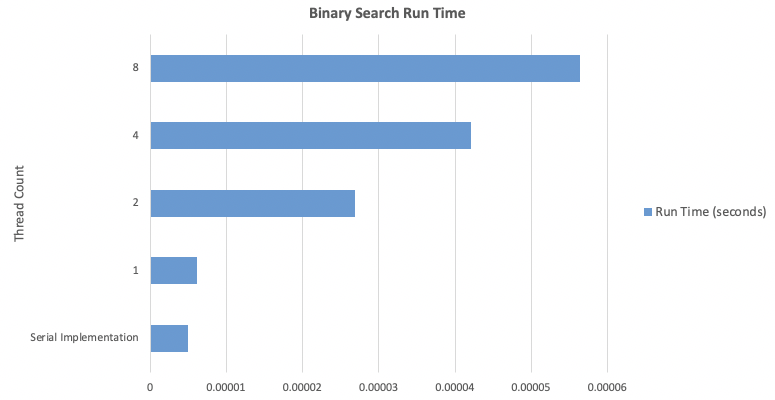
\includegraphics[scale=0.6]{runtime.png}
\vspace*{20px}

\begin{table}[hbt!]
\begin{minipage}[b]{80mm}
\begin{tabular}{@{}ll@{}}
\toprule
\textbf{Thread Count} & \textbf{Run time (seconds)} \\ \midrule
1 (Serial)            & $\sim$0.000005  \\
\bottomrule
\\
\\
\\
\\
\end{tabular}
    \caption{Serial Binary Search Timing}
\end{minipage}
\begin{minipage}[b]{80mm}
\begin{tabular}{@{}ll@{}}
\toprule
\textbf{Thread Count} & \textbf{Run time (seconds)} \\ \midrule
1                     & 0.0000061            \\ \midrule
2                     & 0.0000269            \\ \midrule
4                     & 0.0000421            \\ \midrule
8                     & 0.0000564          \\
\bottomrule
\end{tabular}
    \caption{Parallel Binary Search Timing}
\end{minipage}
\end{table}

\\
\section{Analysis}

\begin{table}[hbt!]
\begin{tabular}{@{}ll@{}}
\toprule
\textbf{Parallel Time Complexity}                & $\mathcal{O}(log{}(n/k))$ \\ \midrule
\textbf{Speedup Estimate}                        & $\frac{log(n^2)}{k}$      \\ \midrule
\textbf{Efficiency Estimate}                     & $\frac{log(n^2)}{k^2}$    \\
\bottomrule
\end{tabular}
    \caption{Theoretical Estimates of Parallel Binary Search}
\end{table}

\subsection*{Real-World Results}
Referring to the data displayed in Table 2 and Table 3, the serial implementation of Binary Search is significantly faster than the parallel implementation. As the number of threads performing Binary Search increased, the operation took exponentially longer. There are a few reasons I can hypothesize as to why these results occurred.

\subsubsection*{Effectivity Limits of Parallel Solutions}
One crucial idea to note, when finding a parallel approach to a problem, is that the serial operation needs to be costly enough to computer resources to parallelize. Often times, complex calculations such as matrix multiplication or dot product are used to demonstrate parallel effectivity, for a specific reason. That is, the operation needs to be costly enough to outweigh the performance repercussions of a parallel solution. Specific performance repercussions such as thread spawning, excessive function calls, voltage and thermal limitations across several threads, and cache hierarchy issues can all play a part in slowing down performance. In the case of Binary Search, the operation simply is not costly enough to make useful out of a parallel approach. OpenMP is not a solution to all problems.



\section{Implementation}
\subsection*{Building and Running This Application}
To build the project and run experiments with it:
\begin{enumerate}
  \item cd into project directory
  \item Run the integer generator, which will output all integer data into input1.txt
  \item Compile the C file
  \item Run the compiled file
\end{enumerate}
\\
\begin{lstlisting}[language=bash]
> cd openmp-binary-search
> python3 integer_generator.py
> clang -Xpreprocessor -fopenmp -lomp binarySearch_openmp.c -o binarySearch_openmp
> ./binarySearch_openmp
\end{lstlisting}


\subsection*{Running Experiments}
There are several factors which need to be accounted for before running experiments and gathering data for a similar program:
\\
\begin{itemize}
  \item Ensure multiple data points are calculated for averaging
  \item Ensure you are running costly enough operations
  \item Ensure operation data set is large enough 
  \item Keep aware that high-resolution timers are not always fully accurate for each floating point
  \item Therefore, do research before choosing a timer
  \item Create a stable thermal environment for the CPU before collecting data
\end{itemize}
\\
After following the above awareness points, the data collection goes as follows:
\\
\begin{enumerate}
  \item Generate all numbers using the random number generator
  \item Pick several numbers of threads in powers of 2
  \item Run the program with each thread count, four times total
  \item Average out each run
  \item Use the average as the calculated run time
\end{enumerate}
\\




\pagebreak
\section{Code Appendix}

\lstinputlisting[language=C, caption=$binarySearch\_openMP.c$]{binarySearch_openmp.c}
\pagebreak
\lstinputlisting[language=Python, caption=$integer\_generator.py$]{integer_generator.py}

\end{document}